\documentclass{beamer}
\usetheme{ucl}

\newcommand\hmmax{0}
\newcommand\bmmax{0}

\usepackage{graphicx}%
\usepackage{multirow}%
\usepackage{amsmath,amssymb,amsfonts}%
%\usepackage{amsthm}%
\usepackage{stmaryrd}
\usepackage{mathrsfs}%
\usepackage[title]{appendix}%
\usepackage{xcolor}%
\usepackage{textcomp}%
\usepackage{manyfoot}%
\usepackage{booktabs}%
\usepackage{algorithm}%
\usepackage{algorithmicx}%
\usepackage{algpseudocode}%
\usepackage{listings}%
\usepackage{orcidlink}
\usepackage{comment}
%%%%
\usepackage{mathtools}  % For cases
%\usepackage{thm-restate}
%\usepackage{mathrsfs}
%\usepackage[inline]{enumitem} %For enum*

\usepackage{mathbbol}
%\usepackage{tikz-cd} % For tikz art
%\usepackage{tikzit}
%\usepackage{ebproof}
\usepackage{bussproofs}
\usepackage{proof}


%%%%%%%%%%%%%%%%%%%%%%%%%%%%%%%%%%%%%%%%%%%%%%%%%%%%%%
%%%%%%%%%%%%%% Define the new environments here;
%\newenvironment{qparts}{\begin{enumerate}[{(}a{)}]}{\end{enumerate}}
% \def\endproofmark{$\Box$}
%\renewenvironment{proof}{\par{\bf Proof}:}{\hfill$\blacksquare$}

\newtheorem{defn}[theorem]{Definition}

\newtheorem{question}[theorem]{Question}
\newtheorem{remark}[theorem]{Remark}
\newtheorem{construction}[theorem]{Construction}
\newtheorem{observation}[theorem]{Observation}

%Make font sans-serif
\renewcommand{\familydefault}{\sfdefault}

%%%%%% Define commands here;

% Basic logic notation.
%\newcommand{\seq}{\triangleright}
\newcommand{\seq}{\Rightarrow }
\newcommand{\sequent}[2]{{#1} \seq {#2}}
\newcommand{\thmSequent}[2]{{#1} \vdash {#2}}

%%%%%%%%%%%%%%%%%%%%%%%%%%%%%%%%%%%%%%%%%
%       BeS
%%%%%%%%%%%%%%%%%%%%%%%%%%%%%%%%%%%%%%%%%
\newcommand{\base}[1]{\mathscr{#1}}
\newcommand{\baseB}{\base{B}}
\newcommand{\baseC}{\base{C}}
\newcommand{\baseD}{\base{D}}
\newcommand{\baseE}{\base{E}}
\newcommand{\baseF}{\base{F}}
\newcommand{\baseG}{\base{G}}
\newcommand{\baseH}{\base{H}}
\newcommand{\baseX}{\base{X}}
\newcommand{\baseY}{\base{Y}}
\newcommand{\baseZ}{\base{Z}}
\newcommand{\baseILL}{\base{N}}
\newcommand{\emptybase}{\varnothing}
\newcommand{\basis}[1]{\mathfrak{#1}}
% \newcommand{\at}[1]{\mathrm{#1}}
\newcommand{\at}[1]{{#1}}
\newcommand{\At}{\mathbb{A}}

%\newcommand{\baseGeq}{\succeq}
%\newcommand{\baseLeq}{\preceq}
\newcommand{\baseGeq}{\supseteq}
\newcommand{\baseLeq}{\subseteq}

\newcommand{\suppTor}[1]{\Vdash_{\!\!#1}}
% \newcommand{\supp}[1]{\Vdash_{\!\!#1}}
% \newcommand{\suppNew}[1]{\vDash_{\!#1}}
\newcommand{\suppNew}[1]{\Vdash^{*}_{\!#1}}
\newcommand{\entails}{\Vdash}
%\newcommand{\proves}[1]{\vdash_{\!\!#1}}
\newcommand{\proves}{\vdash}
\newcommand{\plus}{+}
\newcommand{\system}[1]{\mathsf{#1}}
\newcommand{\Atoms}{\set{A}}
\newcommand{\Formulas}{\set{F}}
\newcommand{\Bunches}{\set{B}}
\newcommand{\set}[1]{\mathbb{#1}}


%%%% ILL
\newcommand{\IPL}{IPL}
\newcommand{\IMLL}{IMLL}
\newcommand{\IMALL}{IMALL}
\newcommand{\ILL}{ILL}
%\newcommand{\provesIMALL}{\vdash_{\mathrm{IMALL}}}
%\newcommand{\provesILL}{\vdash_{\mathrm{ILL}}}
\newcommand{\provesILL}{\vdash}
\newcommand{\multiset}{\mathcal{M}}
\newcommand{\fmultiset}{\mathcal{M}_{\!{f}}}
\newcommand{\emptymultiset}{\varnothing}
\newcommand{\deriveBaseM}[1]{\vdash_{\!\!#1}}
\newcommand{\deriveBaseIPL}[1]{\vdash_{\!\!#1}^{\mathfrak{S}}}
\newcommand{\suppIPL}[1]{\Vdash_{ \!\!#1 }^{\!\!\mathfrak{S}}}
\newcommand{\suppM}[2]{\Vdash_{ \!\!#1 }^{ \!\!#2 }}
\newcommand{\suppIPLAlt}[2]{\Vvdash_{ \!\!#1 }^{ \!\!#2 }}
\newcommand{\suppMAlt}[2]{\Vvdash_{ \!\!#1 }^{ \!\!#2 }}
\newcommand{\suppL}[3]{\Vdash_{ \!\!#1 }^{{ \!\!#2 }\ctxt\hspace*{0.08cm}{ \!\!#3 }}}
%\newcommand{\IMALLformula}{\mathsf{Form}}
\newcommand{\ILLformula}{\mathsf{Form}}
\newcommand{\mand}{\otimes}
\newcommand{\mtop}{1}
\newcommand{\mto}{\multimap}
\newcommand{\aand}{\mathbin{\&}}
\newcommand{\aor}{\oplus}
\newcommand{\abot}{0}
\newcommand{\msetunion}{,}
\newcommand{\bang}{\mathop{!}}
\newcommand{\makeMultiset}[1]{\{#1\}}
\newcommand{\flatILL}[1]{{#1}^{\flat}}
\newcommand{\deflatILL}[1]{{#1}^{\natural}}
\newcommand{\openaddrule}{\{}
\newcommand{\closeaddrule}{\}}
\newcommand{\Closeaddrule}[2]{\}^{#2}_{#1}}
\newcommand{\extAt}{\widetilde{\At}}
\DeclareMathSymbol{\msetsum}{\mathrel}{bbold}{\lq\,}
%\newcommand{\lbang}{\mathop{!}}
\newcommand{\ctxt}{;}
\newcommand{\iplill}[1]{(#1)^\star}
\newcommand{\illipl}[1]{(#1)_\star}



\setbeamersize{description width=2em}
%%% Remove nav symbols (and shift any logo down to corner)
\setbeamertemplate{navigation symbols}{\vspace{-2ex}}
\setbeamertemplate{footline}[author title date]
\setbeamercolor{banner}{bg=darkpurple}
\useinnertheme{blockborder}

\graphicspath{{./images/} }
\title[P-tS for ILL]{Base-extension semantics for Intuitionistic Linear Logic}
%\author{\texorpdfstring{Yll Buzoku\newline\url{y.buzoku@ucl.ac.uk}}{https://www.homepages.ucl.ac.uk/~zcapybu/}}
\author{Yll Buzoku}
\institute[UCL]{%
  Department of Computer Science \\ %
  University College London
}
\date{August 2, 2024}

\AtBeginSection[]
{
  \begin{frame}
    \frametitle{Presentation root directory}
    \tableofcontents[currentsection]
  \end{frame}
}

\begin{document}
%%%%%%%%%%%%%%%%%%%%%%%%%%%%%%%%%%%%%%%%%%%%%%%%%%%%%%%%
%%%%%%%%%%%%%%%%%%%%%%%%%%%%%%%%%%%%%%%%%%%%%%%%%%%%%%%%
\begin{frame}
\titlepage
\end{frame}
%%%%%%%%%%%%%%%%%%%%%%%%%%%%%%%%%%%%%%%%%%%%%%%%%%%%%%%%
%%%%%%%%%%%%%%%%%%%%%%%%%%%%%%%%%%%%%%%%%%%%%%%%%%%%%%%%
\section*{Goals for this presentation}
\begin{frame}{Goals for this talk}
\begin{itemize}%[label={-}]
\item To introduce Intuitionistic Linear Logic and a natural deduction system for it.
\item Present a Base-extension semantics for Intuitionistic Linear Logic.
\item Talk about some of the difficulties involved the process of developing such a semantics.
\end{itemize}
\end{frame}
%%%%%%%%%%%%%%%%%%%%%%%%%%%%%%%%%%%%%%%%%%%%%%%%%%%%%%%%
%%%%%%%%%%%%%%%%%%%%%%%%%%%%%%%%%%%%%%%%%%%%%%%%%%%%%%%%
\begin{frame}{Presentation root directory}
\tableofcontents
\end{frame}
%%%%%%%%%%%%%%%%%%%%%%%%%%%%%%%%%%%%%%%%%%%%%%%%%%%%%%%%
%%%%%%%%%%%%%%%%%%%%%%%%%%%%%%%%%%%%%%%%%%%%%%%%%%%%%%%%
\section{Overview of Intuitionistic Linear Logic}
\begin{frame}{Notation}
	\begin{itemize}%[label={-}]
		\item $\At$ represents a fixed, countably infinite set of propositional atoms. 
		\item Lower case latin letters represent propositional atoms.
		\item Upper case latin letters represent finite multisets of propositional atoms. 
		\item Atomic multiset is taken to mean multiset of propositional atoms.
		\item The sum of two multisets $\at{P}$ and $\at{Q}$ is denoted $\at{P}\msetsum\at{Q}$. 
		\item Lower case greek letters represent ILL formulas.
		\item Upper case greek letters represent ILL finite multisets thereof. 
	\end{itemize}
\end{frame}
%%%%%%%%%%%%%%%%%%%%%%%%%%%%%%%%%%%%%%%%%%%%%%%%%%%%%%%%
\begin{frame}{Formulas of Intuitionistic Linear Logic}
	\begin{definition}
		Formulas of \ILL{} are defined inductively as follows: 
		\[
			\ILLformula \ni \varphi, \psi ::= p \in \At \mid \top \mid \abot \mid \mtop \mid \varphi \mto \psi \mid \varphi \mand \psi \mid \varphi \aand \psi \mid \varphi \aor \psi \mid \bang \varphi
		\]
	\end{definition}
	\pause
	\begin{definition}[Sequent]
		A sequent is a pair $(\Gamma, \varphi)$.
	\end{definition}
	\pause
	\begin{center}
		An example ILL sequent is $(\makeMultiset{\varphi, \varphi \mto \psi}, \psi\mand\chi)$
	\end{center}
\end{frame}
%%%%%%%%%%%%%%%%%%%%%%%%%%%%%%%%%%%%%%%%%%%%%%%%%%%%%%%%
\begin{frame}{A natural deduction system for ILL}
\begin{center}
\noindent\begin{minipage}{0.47\textwidth}\scriptsize
\begin{prooftree}
  \def\ScoreOverhang{0.5pt}
  	\AxiomC{}
  	\RightLabel{Ax}
  	\UnaryInfC{$\varphi\proves\varphi$}
\end{prooftree}
\end{minipage}
\vspace{2pt}
\noindent\begin{minipage}{0.47\textwidth}\scriptsize
	\begin{prooftree}
  	\def\ScoreOverhang{0.5pt}
  		\AxiomC{$\Gamma\msetsum\varphi \proves \psi$}
  		\RightLabel{$\mto$-I}
  		\UnaryInfC{$\Gamma \proves \varphi \mto \psi$}
	\end{prooftree}
	\begin{prooftree}
	\def\ScoreOverhang{0.5pt}
		\AxiomC{$\Gamma \proves \varphi$}
		\AxiomC{$\Delta \proves \psi$}
		\RightLabel{$\mand$-I}
		\BinaryInfC{$\Gamma\msetsum\Delta \proves \varphi\mand\psi$}
	\end{prooftree}
	\begin{prooftree}
	\def\ScoreOverhang{0.5pt}
		\AxiomC{}
		\RightLabel{$\mtop$-I}
		\UnaryInfC{$\proves \mtop$}
	\end{prooftree}
	\begin{prooftree}
	\def\ScoreOverhang{0.5pt}
		\AxiomC{$\Gamma \proves \varphi$}
		\AxiomC{$\Gamma \proves \psi$}
		\RightLabel{$\aand$-I}
		\BinaryInfC{$\Gamma \proves \varphi \aand \psi$}
	\end{prooftree}
	\begin{prooftree}
	\def\ScoreOverhang{0.5pt}
		\AxiomC{$\Gamma \proves \varphi_i$}
		\RightLabel{$\aor$-$\text{I}_i$}
		\UnaryInfC{$\Gamma \proves \varphi_0 \aor \varphi_1$}
	\end{prooftree}
	\begin{prooftree}
		\def\ScoreOverhang{0.5pt}
			\AxiomC{$\Gamma_1 \provesILL \varphi_1$}
			\AxiomC{$\dots$}
			\AxiomC{$\Gamma_n \provesILL \varphi_n$}
			\RightLabel{$\top$-I}
			\TrinaryInfC{$\Gamma_1,\dots,\Gamma_n \provesILL \top$}
		\end{prooftree}
\end{minipage}%%%%%%%%%%%%%%%%%%%%%%%%%%%%%%%%
\begin{minipage}{0.47\textwidth}\scriptsize
	\begin{prooftree}
  	\def\ScoreOverhang{0.5pt}
  		\AxiomC{$\Gamma \proves \varphi \mto \psi$}
  		\AxiomC{$\Delta \proves \varphi$}
  		\RightLabel{$\mto$-E}
  		\BinaryInfC{$\Gamma\msetsum\Delta \proves \psi$}
	\end{prooftree}
	\begin{prooftree}
	\def\ScoreOverhang{0.5pt}
		\AxiomC{$\Gamma \proves \varphi\mand\psi$}
		\AxiomC{$\Delta\msetsum \varphi\msetsum \psi \proves \chi$}
		\RightLabel{$\mand$-E}
		\BinaryInfC{$\Gamma\msetsum\Delta \proves \chi$}
	\end{prooftree}
	\begin{prooftree}
	\def\ScoreOverhang{0.5pt}
		\AxiomC{$\Gamma \proves \varphi$}
		\AxiomC{$\Delta \proves \mtop$}
		\RightLabel{$\mtop$-E}
		\BinaryInfC{$\Gamma\msetsum\Delta \proves \varphi$}
	\end{prooftree}
	\begin{prooftree}
	\def\ScoreOverhang{0.5pt}
		\AxiomC{$\Gamma \proves \varphi_0 \aand \varphi_1$}
		\RightLabel{$\aand$-$\text{E}_i$}
		\UnaryInfC{$\Gamma \proves \varphi_i$}
	\end{prooftree}
	\begin{prooftree}
	\def\ScoreOverhang{0.5pt}
		\AxiomC{$\Gamma \proves \varphi \aor \psi$}
		\AxiomC{$\Delta\msetsum\varphi \proves \chi$}
		\AxiomC{$\Delta\msetsum\psi \proves \chi$}
		\RightLabel{$\aor$-E}
		\TrinaryInfC{$\Gamma\msetsum\Delta \proves \chi$}
	\end{prooftree}
	\begin{prooftree}
	\def\ScoreOverhang{0.5pt}
		\AxiomC{$\Gamma \proves \abot$}
		\RightLabel{$\abot$-E}
		\UnaryInfC{$\Gamma \proves \varphi$}
	\end{prooftree}
\end{minipage}
\end{center}
\end{frame}
%%%%%%%%%%%%%%%%%%%%%%%%%%%%%%%%%%%%%%%%%%%%%%%%%%%%%%%%
\begin{frame}{A natural deduction system for ILL (cont.)}
\begin{center}
\begin{minipage}{0.75\textwidth}\scriptsize
	\begin{prooftree}
		\def\ScoreOverhang{0.5pt}
			\AxiomC{$\Gamma_1 \provesILL \bang\psi_1$}
			\AxiomC{$\ldots$}
			\AxiomC{$\Gamma_n \provesILL \bang\psi_n$}
			\AxiomC{$\bang\psi_1\msetsum\ldots\msetsum \bang\psi_n \provesILL \varphi$}
			\RightLabel{$\bang$-Promotion}
			\QuaternaryInfC{$\Gamma_1\msetsum\ldots\msetsum\Gamma_n \provesILL \bang\varphi$}
	\end{prooftree}
	\begin{prooftree}
		\def\ScoreOverhang{0.5pt}
			\AxiomC{$\Gamma \provesILL \bang\varphi$}
			\AxiomC{$\Delta\msetsum \varphi \provesILL \psi$}
			\RightLabel{$\bang$-Dereliction}
			\BinaryInfC{$\Gamma\msetsum\Delta\provesILL \psi$}
	\end{prooftree}
	\begin{prooftree}
		\def\ScoreOverhang{0.5pt}
			\AxiomC{$\Gamma \provesILL \bang\varphi$}
			\AxiomC{$\Delta \provesILL \psi$}
			\RightLabel{$\bang$-Weakening}
			\BinaryInfC{$\Gamma\msetsum\Delta\provesILL \psi$}
	\end{prooftree}
	\begin{prooftree}
		\def\ScoreOverhang{0.5pt}
			\AxiomC{$\Gamma \provesILL \bang\varphi$}
			\AxiomC{$\Delta\msetsum\bang\varphi\msetsum\bang\varphi \provesILL \psi$}
			\RightLabel{$\bang$-Contraction}
			\BinaryInfC{$\Gamma\msetsum\Delta\provesILL \psi$}
	\end{prooftree}
\end{minipage}
\end{center}
\end{frame}
%%%%%%%%%%%%%%%%%%%%%%%%%%%%%%%%%%%%%%%%%%%%%%%%%%%%%%%%
\begin{frame}{What is the general form of an inference figure?}
	\pause
	\begin{prooftree}
		\def\ScoreOverhang{0.5pt}
			\AxiomC{$\Gamma \proves \varphi_1$}
			\AxiomC{$\Delta \proves \varphi_2$}
			\RightLabel{$\mand$-I}
			\BinaryInfC{$\Gamma\msetsum\Delta \proves \varphi_1\mand\varphi_2$}
	\end{prooftree}
\end{frame}
%%%%%%%%%%%%%%%%%%%%%%%%%%%%%%%%%%%%%%%%%%%%%%%%%%%%%%%%
\begin{frame}{What is the general form of an inference figure?}
	\begin{prooftree}
		\def\ScoreOverhang{0.5pt}
			\AxiomC{$\Gamma \proves \varphi_1$}
			\AxiomC{$\Gamma \proves \varphi_2$}
			\RightLabel{$\aand$-I}
			\BinaryInfC{$\Gamma \proves \varphi_1 \aand \varphi_2$}
		\end{prooftree}
\end{frame}
%%%%%%%%%%%%%%%%%%%%%%%%%%%%%%%%%%%%%%%%%%%%%%%%%%%%%%%%
\begin{frame}[b]{What is the general form of an inference figure?}
	\pause
	\begin{minipage}{0.47\textwidth}\scriptsize
		\begin{prooftree}
			\AxiomC{$\Gamma_1 \proves \varphi_1$}
			\AxiomC{$\dots$}
			\AxiomC{$\Gamma_n \proves \varphi_n$}
			\TrinaryInfC{$\Gamma_1\msetsum\dots\msetsum\Gamma_n \proves \psi$}
		\end{prooftree}
	\end{minipage}
	\begin{minipage}{0.47\textwidth}\scriptsize
		\begin{prooftree}
			\AxiomC{$\Gamma \proves \varphi_1$}
			\AxiomC{$\dots$}
			\AxiomC{$\Gamma \proves \varphi_n$}
			\dashedLine
			\TrinaryInfC{$\Gamma \proves \psi$}
		\end{prooftree}
	\end{minipage}
	\vspace{2cm}
	\pause
	\begin{prooftree}
		\def\ScoreOverhang{0.5pt}
			\AxiomC{$\Gamma \proves \varphi_1 \aor \varphi_2$}
			\AxiomC{$\Delta\msetsum\varphi_1 \proves \chi$}
			\AxiomC{$\Delta\msetsum\varphi_2 \proves \chi$}
			\RightLabel{$\aor$-E}
			\TrinaryInfC{$\Gamma\msetsum\Delta \proves \chi$}
	\end{prooftree}
\end{frame}
%%%%%%%%%%%%%%%%%%%%%%%%%%%%%%%%%%%%%%%%%%%%%%%%%%%%%%%%
\begin{frame}{What is the general form of an inference figure?}
	\begin{prooftree}
		\def\ScoreOverhang{0.5pt}
			\AxiomC{$\Gamma \proves \varphi_1 \aor \varphi_2$}
			\AxiomC{$\Delta\msetsum\varphi_1 \proves \chi$}
			\AxiomC{$\Delta\msetsum\varphi_2 \proves \chi$}
			\RightLabel{$\aor$-E}
			\TrinaryInfC{$\Gamma\msetsum\Delta \proves \chi$}
	\end{prooftree}
\end{frame}
%%%%%%%%%%%%%%%%%%%%%%%%%%%%%%%%%%%%%%%%%%%%%%%%%%%%%%%%
\begin{frame}{What is the general form of an inference figure?}
	\begin{prooftree}
		\def\ScoreOverhang{0.5pt}
			\AxiomC{$\Gamma \proves \varphi_1 \aor \varphi_2$}
			\AxiomC{$\Delta\,\openaddrule\varphi_1 \proves \chi$}
			\AxiomC{$\varphi_2 \proves \chi\closeaddrule$}
			\RightLabel{$\aor$-E}
			\TrinaryInfC{$\Gamma\msetsum\Delta \proves \chi$}
	\end{prooftree}
\end{frame}
%%%%%%%%%%%%%%%%%%%%%%%%%%%%%%%%%%%%%%%%%%%%%%%%%%%%%%%%
\begin{frame}{What is the general form of an inference figure?}
	\begin{prooftree}
		\def\ScoreOverhang{0.5pt}
			\AxiomC{$\Gamma\,\openaddrule \emptymultiset\proves \varphi_1 \aor \varphi_2\closeaddrule$}
			\AxiomC{$\Delta\,\openaddrule\varphi_1 \proves \chi$}
			\AxiomC{$\varphi_2 \proves \chi\closeaddrule$}
			\RightLabel{$\aor$-E}
			\TrinaryInfC{$\Gamma\msetsum\Delta \proves \chi$}
	\end{prooftree}
\end{frame}
%%%%%%%%%%%%%%%%%%%%%%%%%%%%%%%%%%%%%%%%%%%%%%%%%%%%%%%%
\begin{frame}{What is the general form of an inference figure?}
	\begin{prooftree}
		\def\ScoreOverhang{0.5pt}
			\AxiomC{$\Gamma\,\openaddrule \emptymultiset\proves \varphi_1 \aor \varphi_2\closeaddrule$}
			\AxiomC{$\Delta\,\openaddrule\varphi_1 \proves \chi$}
			\AxiomC{$\varphi_2 \proves \chi\closeaddrule$}
			\RightLabel{$\aor$-E}
			\TrinaryInfC{$\Gamma\msetsum\Delta \proves \chi$}
	\end{prooftree}
\end{frame}
%%%%%%%%%%%%%%%%%%%%%%%%%%%%%%%%%%%%%%%%%%%%%%%%%%%%%%%%
\begin{frame}{What is the general form of an inference figure?}
	\begin{prooftree}
		\def\ScoreOverhang{0.5pt}
			\AxiomC{$\Gamma\, \openaddrule\emptymultiset\proves \varphi_1\closeaddrule$}
			\AxiomC{$\Delta\, \openaddrule\emptymultiset\proves \varphi_2\closeaddrule$}
			\RightLabel{$\mand$-I}
			\BinaryInfC{$\Gamma\msetsum\Delta \proves \varphi_1\mand\varphi_2$}
	\end{prooftree}
	\vspace{1cm}
	\begin{prooftree}
		\def\ScoreOverhang{0.5pt}
			\AxiomC{$\Gamma\,\openaddrule \emptymultiset\proves \varphi_1$}
			\AxiomC{$\emptymultiset \proves \varphi_2\closeaddrule$}
			\RightLabel{$\aand$-I}
			\BinaryInfC{$\Gamma \proves \varphi_1 \aand \varphi_2$}
		\end{prooftree}
\end{frame}
%%%%%%%%%%%%%%%%%%%%%%%%%%%%%%%%%%%%%%%%%%%%%%%%%%%%%%%%
\begin{frame}{What is the general form of an inference figure?}
		\begin{prooftree}
			\AxiomC{$\dots$}
			\AxiomC{$\Gamma_i\hspace*{5pt}\openaddrule \Delta_{i_1}\proves \varphi_{i_1}$}
			\AxiomC{$\dots$}
			\AxiomC{$\Delta_{i_{l_i}}\proves \varphi_{i_{l_i}}\closeaddrule$}
			\AxiomC{$\dots$}
			\QuinaryInfC{$\Gamma_1\msetsum\dots\msetsum\Gamma_n \proves \psi$}
		\end{prooftree}
\end{frame}
%%%%%%%%%%%%%%%%%%%%%%%%%%%%%%%%%%%%%%%%%%%%%%%%%%%%%%%%
\begin{frame}{What is the general form of an inference figure?}
	\pause
	Almost! What about:\newline
	\begin{prooftree}
		\def\ScoreOverhang{0.5pt}
			\AxiomC{$\Gamma_1 \provesILL \bang\psi_1$}
			\AxiomC{$\ldots$}
			\AxiomC{$\Gamma_n \provesILL \bang\psi_n$}
			\AxiomC{$\bang\psi_1\msetsum\ldots\msetsum \bang\psi_n \provesILL \varphi$}
			\RightLabel{$\bang$-Promotion}
			\QuaternaryInfC{$\Gamma_1\msetsum\ldots\msetsum\Gamma_n \provesILL \bang\varphi$}
	\end{prooftree}
\end{frame}
%%%%%%%%%%%%%%%%%%%%%%%%%%%%%%%%%%%%%%%%%%%%%%%%%%%%%%%%
\begin{frame}{What is the general form of an inference figure?}
	\begin{prooftree}
		\def\ScoreOverhang{0.5pt}
			\AxiomC{$\Gamma_1\, \openaddrule\emptymultiset\provesILL \bang\psi_1\closeaddrule$}
			\AxiomC{$\ldots$}
			\AxiomC{$\Gamma_n\, \openaddrule\emptymultiset\provesILL \bang\psi_n\closeaddrule$}
			\AxiomC{$\bang\psi_1\msetsum\ldots\msetsum \bang\psi_n \provesILL \varphi$}
			\RightLabel{$\bang$-Promotion}
			\QuaternaryInfC{$\Gamma_1\msetsum\ldots\msetsum\Gamma_n \provesILL \bang\varphi$}
	\end{prooftree}
\end{frame}
%%%%%%%%%%%%%%%%%%%%%%%%%%%%%%%%%%%%%%%%%%%%%%%%%%%%%%%%
%%%%%%%%%%%%%%%%%%%%%%%%%%%%%%%%%%%%%%%%%%%%%%%%%%%%%%%%
\section{Base-extension Semantics for ILL}
\begin{frame}{Substructural atomic derivability}
\begin{definition}[Basic rule]
Basic rules take the following form: 
\[\openaddrule (\at{P}_{1_i} \seq \at{q}_{1_i})\closeaddrule^{l_1}_{i=1}, \dots, \openaddrule (\at{P}_{n_i} \seq \at{q}_{n_i})\closeaddrule^{l_n}_{i=1} \Rightarrow \at{r}\]
\end{definition}
%
\begin{itemize}
	\item Each $(P_i \seq q_i)$ is a pair $(P_i, q_i)$ called an atomic sequent.
	\item Each collection $\openaddrule (\at{P}_{i_1} \seq \at{q}_{i_1}), \dots, (\at{P}_{i_{l_i}} \seq \at{q}_{i_{l_i}})\closeaddrule$ is called an atomic box.
\end{itemize}
\pause
\begin{definition}[Base]
	A base $\baseB$ is a $\mathbf{SET}$ of basic rules. 
\end{definition}
\end{frame}
%%%%%%%%%%%%%%%%%%%%%%%%%%%%%%%%%%%%%%%%%%%%%%%%%%%%%%%%
\begin{frame}{Substructural atomic derivability}
\begin{definition}[Basic derivability relation]
The relation of derivability in a base $\baseB$, is defined inductively as so:
\begin{itemize}
\item[Ref] $p \deriveBaseM{\baseB} p$
\item[App] Given that $(\openaddrule(\at{P}_{1_i} \seq \at{q}_{1_{i}})\Closeaddrule{i=1}{l_1},\dots,\openaddrule(\at{P}_{n_i} \seq \at{q}_{n_{i}}) \Closeaddrule{i=1}{l_n} \Rightarrow \at{r}) \in \baseB$ and atomic multisets $\at{C}_i$ such that the following hold:
        \[\at{C}_i\msetsum\at{P}_{i_j} \deriveBaseM{\baseB} \at{q}_{i_j} \text{ for all } i = 1,\dots, n \text{ and } j = 1,\dots,l_i\]
Then $\at{C}_{1}\msetsum\ldots\msetsum\at{C}_{n}\deriveBaseM{\baseB} r$. 
\end{itemize}
\end{definition}
\end{frame}
%%%%%%%%%%%%%%%%%%%%%%%%%%%%%%%%%%%%%%%%%%%%%%%%%%%%%%%%
\begin{frame}{Example derivations}
	\begin{example}[Derivation terminations]
		Let $\baseB=\{(\Rightarrow a), (\openaddrule \Rightarrow a \closeaddrule,\openaddrule\Rightarrow b\closeaddrule\Rightarrow c)\}$
		\begin{prooftree}
			\AxiomC{}
			\RightLabel{Ref}
			\UnaryInfC{$b\deriveBaseM{\baseB}b$}
			\AxiomC{}
			\RightLabel{$\Rightarrow a$}
			\UnaryInfC{$\deriveBaseM{\baseB}a$}
			\RightLabel{$\openaddrule \Rightarrow a \closeaddrule,\openaddrule\Rightarrow b\closeaddrule\Rightarrow c$}
			\BinaryInfC{$b\deriveBaseM{\baseB}c$}
		\end{prooftree}
		Therefore, in $\baseB$, the atom $c$ is derivable from $b$. 
	\end{example}
\end{frame}
%%%%%%%%%%%%%%%%%%%%%%%%%%%%%%%%%%%%%%%%%%%%%%%%%%%%%%%%
\begin{frame}{Example derivations}
	\begin{example}[Invalid derivation]
		By the definition of $\deriveBaseM{\baseB}$, deriving $a$ from $a\msetsum a$ in the empty base is not possible, i.e. $a\msetsum a\deriveBaseM{\emptybase}a$ is not possible.
	\end{example}
	\pause
	\begin{example}[Invalid derivation 2]
		Let $\baseB=\{(\openaddrule\Rightarrow a\closeaddrule\Rightarrow c), (\openaddrule a\Rightarrow c\closeaddrule\Rightarrow b)\}$
		\begin{prooftree}
			\AxiomC{$\times$}
			\UnaryInfC{$a\msetsum a\deriveBaseM{\baseB}a$}
			\RightLabel{$\openaddrule\Rightarrow a\closeaddrule\Rightarrow c$}
			\UnaryInfC{$a\msetsum a\deriveBaseM{\baseB}c$}
			\RightLabel{$\openaddrule a\Rightarrow c\closeaddrule\Rightarrow b$}
			\UnaryInfC{$a\deriveBaseM{\baseB}b$}
		\end{prooftree}
		We see that in this base, $a$ is not derivable from $a\msetsum a$.
	\end{example}
\end{frame}
%%%%%%%%%%%%%%%%%%%%%%%%%%%%%%%%%%%%%%%%%%%%%%%%%%%%%%%%
\begin{frame}{Example derivations}
	\begin{example}[A possible fix for invalid derivation 2]
		Let $\baseC=\{(\openaddrule \Rightarrow a\closeaddrule\Rightarrow c), (\openaddrule a\Rightarrow c\closeaddrule\Rightarrow b),(\openaddrule\Rightarrow a\closeaddrule,\openaddrule\Rightarrow a\closeaddrule\Rightarrow a)\}$
		\begin{prooftree}
			\AxiomC{}
			\RightLabel{Ref}
			\UnaryInfC{$a\deriveBaseM{\baseC}a$}			
			\AxiomC{}
			\RightLabel{Ref}
			\UnaryInfC{$a\deriveBaseM{\baseC}a$}
			\RightLabel{$\openaddrule\Rightarrow a\closeaddrule,\openaddrule\Rightarrow a\closeaddrule\Rightarrow a$}
			\BinaryInfC{$a\msetsum a\deriveBaseM{\baseC}a$}
			\RightLabel{$\openaddrule \Rightarrow a\closeaddrule\Rightarrow c$}
			\UnaryInfC{$a\msetsum a\deriveBaseM{\baseC}c$}
			\RightLabel{$\openaddrule a\Rightarrow c\closeaddrule\Rightarrow b$}
			\UnaryInfC{$a\deriveBaseM{\baseC}b$}
		\end{prooftree}
		Note that $\baseC\supset\baseB$\hspace{5pt}!!
	\end{example}
\end{frame}
%%%%%%%%%%%%%%%%%%%%%%%%%%%%%%%%%%%%%%%%%%%%%%%%%%%%%%%%
\begin{frame}{Example derivations}
	\begin{example}[Another possible fix for invalid derivation 2]
		Let $\baseD=\{(\openaddrule \Rightarrow a\closeaddrule\Rightarrow c), (\openaddrule a\Rightarrow c\closeaddrule\Rightarrow b),(\openaddrule\Rightarrow d\closeaddrule,\openaddrule\Rightarrow d\closeaddrule\Rightarrow a),(\openaddrule\Rightarrow a\closeaddrule\Rightarrow d)\}$
		\begin{prooftree}
			\AxiomC{}
			\RightLabel{Ref}
			\UnaryInfC{$a\deriveBaseM{\baseD}a$}
			\RightLabel{$\openaddrule\Rightarrow a\closeaddrule\Rightarrow d$}
			\UnaryInfC{$a\deriveBaseM{\baseD}d$}
			\AxiomC{}
			\RightLabel{Ref}
			\UnaryInfC{$a\deriveBaseM{\baseD}a$}			
			\RightLabel{$\openaddrule\Rightarrow a\closeaddrule\Rightarrow d$}
			\UnaryInfC{$a\deriveBaseM{\baseD}d$}
			\RightLabel{$\openaddrule\Rightarrow d\closeaddrule,\openaddrule\Rightarrow d\closeaddrule\Rightarrow a$}
			\BinaryInfC{$a\msetsum a\deriveBaseM{\baseD}a$}
			\RightLabel{$\openaddrule \Rightarrow a\closeaddrule\Rightarrow c$}
			\UnaryInfC{$a\msetsum a\deriveBaseM{\baseD}c$}
			\RightLabel{$\openaddrule a\Rightarrow c\closeaddrule\Rightarrow b$}
			\UnaryInfC{$a\deriveBaseM{\baseD}b$}
		\end{prooftree}
	\end{example}
\end{frame}
%%%%%%%%%%%%%%%%%%%%%%%%%%%%%%%%%%%%%%%%%%%%%%%%%%%%%%%%
\begin{frame}{Example derivations}
	\begin{example}[A live complicated derivation!]
		Consider a base $\baseB$ with only the following rules:
		\begin{itemize}
			\item $\openaddrule\Rightarrow c\closeaddrule,\openaddrule\Rightarrow y\closeaddrule\Rightarrow f$
			\item $\Rightarrow z$
			\item $\openaddrule \Rightarrow a\closeaddrule,\openaddrule \Rightarrow b\closeaddrule,\openaddrule\Rightarrow z\closeaddrule\Rightarrow h$
			\item $\openaddrule\Rightarrow h\closeaddrule\Rightarrow g$
			\item $\openaddrule\Rightarrow x\closeaddrule,\openaddrule\Rightarrow g\closeaddrule\Rightarrow e$
			\item $\openaddrule x\Rightarrow e\closeaddrule,\openaddrule y\Rightarrow f\closeaddrule\Rightarrow d$
		\end{itemize}
		is there a derivation of $d$ from the multiset $a\msetsum b\msetsum c$ in $\baseB$?
%		\begin{prooftree}
%			\AxiomC{}
%			\RightLabel{Ref}
%			\UnaryInfC{$f\deriveBaseM{\baseB}f$}
%			\AxiomC{}
%			\RightLabel{Ref}
%			\UnaryInfC{$c\deriveBaseM{\baseB}c$}
%			\RightLabel{$\openaddrule\Rightarrow c\closeaddrule,\openaddrule\Rightarrow y\closeaddrule\Rightarrow f$}
%			\BinaryInfC{$c,y\deriveBaseM{\baseB}f$}
%			\AxiomC{}
%			\RightLabel{$\Rightarrow z$}
%			\UnaryInfC{$\deriveBaseM{\baseB}z$}
%			\AxiomC{}
%			\RightLabel{Inf}
%			\UnaryInfC{$b\deriveBaseM{\baseB}b$}
%			\AxiomC{}
%			\RightLabel{Inf}
%			\UnaryInfC{$a\deriveBaseM{\baseB}a$}
%			\RightLabel{$\openaddrule \Rightarrow a\closeaddrule,\openaddrule \Rightarrow b\closeaddrule,\openaddrule\Rightarrow z\closeaddrule\Rightarrow h$}
%			\TrinaryInfC{$a,b,\deriveBaseM{\baseB}h$}
%			\RightLabel{$\openaddrule\Rightarrow h\closeaddrule\Rightarrow g$}
%			\UnaryInfC{$a,b\deriveBaseM{\baseB}g$}
%			\AxiomC{}
%			\RightLabel{Ref}
%			\UnaryInfC{$x\deriveBaseM{\baseB}x$}
%			\RightLabel{$\openaddrule\Rightarrow x\closeaddrule,\openaddrule\Rightarrow g\closeaddrule\Rightarrow e$}
%			\BinaryInfC{$a,b,x\deriveBaseM{\baseB}e$}
%			\RightLabel{$\openaddrule x\Rightarrow e\closeaddrule,\openaddrule y\Rightarrow f\closeaddrule\Rightarrow d$}
%			\BinaryInfC{$a,b,c\deriveBaseM{\baseB}b$}
%		\end{prooftree}
	\end{example}
	\pause 
	\emph{Disclaimer: The fact I couldn't fit this derivation on the slide has nothing to do with why we are doing this derivation live :-)}
\end{frame}
%%%%%%%%%%%%%%%%%%%%%%%%%%%%%%%%%%%%%%%%%%%%%%%%%%%%%%%%
\begin{frame}{Example derivations}
	\begin{example}[A very interesting derivation]
		Let $\baseB = \{
		(\openaddrule\Rightarrow b\closeaddrule\Rightarrow c),
		(\openaddrule\Rightarrow a\closeaddrule,\openaddrule b\Rightarrow c\closeaddrule\Rightarrow d),
		(\openaddrule\Rightarrow d, \Rightarrow a \closeaddrule\Rightarrow e),
		(\openaddrule a\Rightarrow e\closeaddrule\Rightarrow f)
		\}$
		\begin{prooftree}
			\AxiomC{}
			\RightLabel{Ref}
			\UnaryInfC{$a\deriveBaseM{\baseB}a$}			
			\AxiomC{}
			\RightLabel{Ref}
			\UnaryInfC{$b\deriveBaseM{\baseB}b$}
			\RightLabel{$\openaddrule\Rightarrow b\closeaddrule\Rightarrow c$}
			\UnaryInfC{$b\deriveBaseM{\baseB}c$}
			\RightLabel{$\openaddrule\Rightarrow a\closeaddrule,\openaddrule b\Rightarrow c\closeaddrule\Rightarrow d$}
			\BinaryInfC{$a\deriveBaseM{\baseB}d$}
			\AxiomC{}
			\RightLabel{Ref}
			\UnaryInfC{$a\deriveBaseM{\baseB}a$}
			\RightLabel{$\openaddrule\Rightarrow d, \Rightarrow a \closeaddrule\Rightarrow e$}
			\BinaryInfC{$a\deriveBaseM{\baseB}e$}
			\RightLabel{$\openaddrule a\Rightarrow e\closeaddrule\Rightarrow f$}
			\UnaryInfC{$\deriveBaseM{\baseB}f$}
		\end{prooftree}
	\end{example}
\end{frame}
%%%%%%%%%%%%%%%%%%%%%%%%%%%%%%%%%%%%%%%%%%%%%%%%%%%%%%%%
\begin{frame}{An interesting property of $\deriveBaseM{\baseB}$}
	\begin{lemma}[Substitution lemma]
			The following are equivalent for arbitrary atomic multisets $P\msetsum  S$, atom $q$, and base $\baseB$, where we assume $P = \makeMultiset{p_1,\dots, p_n}$: 
			\begin{itemize}
				\item $P\msetsum  S \deriveBaseM{\baseB} q$
				\item For every $\baseC \baseGeq \baseB$, atomic multisets $T_1, \dots, T_m$ where $T_1 \deriveBaseM{\baseC} p_1, \dots, T_n \deriveBaseM{\baseC} p_m$, then $T_1\msetsum\dots\msetsum T_m\msetsum S \deriveBaseM{\baseC} q$
			\end{itemize}
	\end{lemma}
\end{frame}
%%%%%%%%%%%%%%%%%%%%%%%%%%%%%%%%%%%%%%%%%%%%%%%%%%%%%%%%
\begin{frame}%{Base-extension Semantics for ILL}
	\noindent\begin{minipage}{0.47\textwidth}\scriptsize
		\begin{figure}[t]
			\[
				\begin{array}{r@{\qquad}l@{\quad}c@{\quad}l}
					\mbox{(At)} & \suppM{\baseB}{L} p  & \text{ iff } &   L\deriveBaseM{\baseB} p  \\ [1mm]
					% 
					(\mto) & \suppM{\baseB}{L} \varphi \mto \psi & \text{ iff } & \varphi \suppM{\baseB}{L} \psi \\[1mm]
					% 
					(\mand) & \suppM{\baseB}{L} \varphi \mand \psi   & \text{ iff } &  \text{for any } \baseC  \text{ such that } \baseB \baseLeq \baseC \text{, atomic multisets } K \\ 
					& & & \text{and any } p \in \At, \text{ if } \varphi\msetsum\psi\suppM{\baseB}{K}p \text{ then } \suppM{\baseC}{L\msetsum K} p  \\[1mm]
					%
					(\mtop) & \suppM{\baseB}{L} \mtop   & \text{ iff } &  \text{for any } \baseC  \text{ such that } \baseB \baseLeq \baseC \text{, atomic multisets } K \\ 
					& & & \text{and any } p \in \At, \text{ if } \suppM{\baseB}{K}p \text{ then } \suppM{\baseC}{L\msetsum K} p  \\[1mm]
					%
					(\top) & \suppM{\baseB}{L} \top & \text{ iff } & \text{always} \\[1mm] 
					%
					(\aand) & \suppM{\baseB}{L} \varphi \aand \psi   & \text{ iff } &   \suppM{\baseB}{L} \varphi \text{ and }   \suppM{\baseB}{L} \psi  \\[1mm] 
					%
					(\aor) & \suppM{\baseB}{L} \varphi \aor \psi & \text{ iff } &  \text{for any } \baseC  \text{ such that } \baseB \baseLeq \baseC \text{, atomic multisets } K \\ 
					& & & \text{and any } p \in \At, \text{ if } \varphi \suppM{\baseC}{K} p \text{ and } \psi \suppM{\baseC}{K} p, \text{ then } \suppM{\baseC}{L\msetsum K} p  \\[1mm]
					% 
					(\abot) & \suppM{\baseB}{L} \abot & \text{iff} &    \suppM{\baseB}{L} p \text{ for any } p \in \At \\[1mm]
					%
					(\bang) & \suppM{\baseB}{L} \bang \varphi & \text{iff} &  \text{for any } \baseC  \text{ such that } \baseB \baseLeq \baseC \text{, atomic multisets } K \\ 
					& & & \text{and any } p \in \At, \text{ if for any } \baseD \text{ such that } \baseC\baseLeq\baseD, \\
					& & & (\text{if } \suppM{\baseD}{\emptymultiset}\varphi \text{ then } \suppM{\baseD}{L}p) \text{ then } \suppM{\baseC}{L\msetsum K}p  \\[1mm]
					%
					(\msetsum) & \suppM{\baseB}{L}\Gamma\msetsum\Delta & \text{iff} & \text{there exists multisets } K \text{ and } M \text{ such that } L=K\msetsum M \\ 
					& & &\text{and } \suppM{\baseB}{K}\Gamma \text{ and } \suppM{\baseB}{M}\Delta \\
					%
					\mbox{(Inf)} & \hspace{-1em} \bang\Delta\msetsum\Theta \suppM{\baseB}{L} \varphi & \text{ iff } & \text{for any } \baseC \text{ such that } \baseB \baseLeq \baseC \text{, atomic multisets } K, \\
					& & & \text{if }   \suppM{\baseC}{\emptymultiset} \Delta \text{ and } \suppM{\baseC}{K} \Theta \text{ then } \suppM{\baseC}{L\msetsum K} \varphi \\[1mm]
				\end{array}
			\]
		\end{figure}
	\end{minipage}
\end{frame}
%%%%%%%%%%%%%%%%%%%%%%%%%%%%%%%%%%%%%%%%%%%%%%%%%%%%%%%%
\begin{frame}{Base-extension Semantics for ILL}
	Note the clause for ($\bang$) could be written as:
	\begin{itemize}
		\item $\suppM{\baseB}{L} \bang \varphi$ iff for any $\baseC$ such that $\baseC \baseGeq \baseB$, atomic multisets $K$ and any $\at{p} \in \At$, if $\bang\varphi\suppM{\baseC}{K}\at{p}$ then $\suppM{\baseC}{L,K}\at{p}$.
	\end{itemize}
\end{frame}
%%%%%%%%%%%%%%%%%%%%%%%%%%%%%%%%%%%%%%%%%%%%%%%%%%%%%%%%
\begin{frame}{Notes on $\suppM{\baseB}{\at{L}}$}
	\begin{itemize}
	\item The sequent $(\Gamma,\varphi)$ is said to be valid if and only if $\Gamma\suppM{\emptybase}{\emptymultiset}\varphi$ holds.
	\vspace{5pt}
	\pause
	\item We frequently write this as $\Gamma \suppM{}{}\varphi$.
	\end{itemize}
\end{frame}
%%%%%%%%%%%%%%%%%%%%%%%%%%%%%%%%%%%%%%%%%%%%%%%%%%%%%%%%
\begin{frame}{Notes on $\suppM{\baseB}{\at{L}}$}
\begin{itemize}
	\item If $\suppM{\baseB}{L}\varphi$ then for all $\baseC \baseGeq \baseB$ we have $\suppM{\baseC}{L}\varphi$.
	\vspace{5pt}
	\item Given $\Gamma\suppM{\baseB}{L}\varphi$ and $\suppM{\baseB}{K}\Gamma$, then it holds that $\suppM{\baseB}{L\msetsum K}\varphi$.
%\vspace{5pt}
%\item $\suppM{\baseB}{\at{L}}\varphi$ iff for all $\baseC \baseGeq \baseB$ and atomic multisets $\at{K}$ and atoms $p$,\, $\varphi\suppM{\baseC}{K}p$ implies $\suppM{\baseC}{L,K}p$. 
\end{itemize}
\end{frame}
%%%%%%%%%%%%%%%%%%%%%%%%%%%%%%%%%%%%%%%%%%%%%%%%%%%%%%%%
\begin{frame}{Soundness}
	\begin{theorem}[Soundness]
		\centering
		If $\Gamma\proves\varphi$ then $\Gamma\suppM{}{}\varphi$
	\end{theorem}
	\pause
	\begin{itemize}
		\item The strategy is to show every rule of the natural deduction system presented previously is semantically expressible.
		\item This suffices by induction to prove this theorem as now we can encode any deduction into a series of semantic proofs.
	\end{itemize}
\end{frame}
%%%%%%%%%%%%%%%%%%%%%%%%%%%%%%%%%%%%%%%%%%%%%%%%%%%%%%%%
\begin{frame}{A reminder of the rules of natural deduction for ILL}
	\begin{center}
	\noindent\begin{minipage}{0.47\textwidth}\scriptsize
	\begin{prooftree}
	  \def\ScoreOverhang{0.5pt}
		  \AxiomC{}
		  \RightLabel{Ax}
		  \UnaryInfC{$\varphi\proves\varphi$}
	\end{prooftree}
	\end{minipage}
	\vspace{2pt}
	\noindent\begin{minipage}{0.47\textwidth}\scriptsize
		\begin{prooftree}
		  \def\ScoreOverhang{0.5pt}
			  \AxiomC{$\Gamma\msetsum\varphi \proves \psi$}
			  \RightLabel{$\mto$-I}
			  \UnaryInfC{$\Gamma \proves \varphi \mto \psi$}
		\end{prooftree}
		\begin{prooftree}
		\def\ScoreOverhang{0.5pt}
			\AxiomC{$\Gamma \proves \varphi$}
			\AxiomC{$\Delta \proves \psi$}
			\RightLabel{$\mand$-I}
			\BinaryInfC{$\Gamma\msetsum\Delta \proves \varphi\mand\psi$}
		\end{prooftree}
		\begin{prooftree}
		\def\ScoreOverhang{0.5pt}
			\AxiomC{}
			\RightLabel{$\mtop$-I}
			\UnaryInfC{$\proves \mtop$}
		\end{prooftree}
		\begin{prooftree}
		\def\ScoreOverhang{0.5pt}
			\AxiomC{$\Gamma \proves \varphi$}
			\AxiomC{$\Gamma \proves \psi$}
			\RightLabel{$\aand$-I}
			\BinaryInfC{$\Gamma \proves \varphi \aand \psi$}
		\end{prooftree}
		\begin{prooftree}
		\def\ScoreOverhang{0.5pt}
			\AxiomC{$\Gamma \proves \varphi_i$}
			\RightLabel{$\aor$-$\text{I}_i$}
			\UnaryInfC{$\Gamma \proves \varphi_0 \aor \varphi_1$}
		\end{prooftree}
		\begin{prooftree}
            \def\ScoreOverhang{0.5pt}
                \AxiomC{$\Gamma_1 \provesILL \varphi_1$}
                \AxiomC{$\dots$}
                \AxiomC{$\Gamma_n \provesILL \varphi_n$}
                \RightLabel{$\top$-I}
                \TrinaryInfC{$\Gamma_1,\dots,\Gamma_n \provesILL \top$}
            \end{prooftree}
	\end{minipage}%%%%%%%%%%%%%%%%%%%%%%%%%%%%%%%%
	\begin{minipage}{0.47\textwidth}\scriptsize
		\begin{prooftree}
		  \def\ScoreOverhang{0.5pt}
			  \AxiomC{$\Gamma \proves \varphi \mto \psi$}
			  \AxiomC{$\Delta \proves \varphi$}
			  \RightLabel{$\mto$-E}
			  \BinaryInfC{$\Gamma\msetsum\Delta \proves \psi$}
		\end{prooftree}
		\begin{prooftree}
		\def\ScoreOverhang{0.5pt}
			\AxiomC{$\Gamma \proves \varphi\mand\psi$}
			\AxiomC{$\Delta\msetsum \varphi\msetsum \psi \proves \chi$}
			\RightLabel{$\mand$-E}
			\BinaryInfC{$\Gamma\msetsum\Delta \proves \chi$}
		\end{prooftree}
		\begin{prooftree}
		\def\ScoreOverhang{0.5pt}
			\AxiomC{$\Gamma \proves \varphi$}
			\AxiomC{$\Delta \proves \mtop$}
			\RightLabel{$\mtop$-E}
			\BinaryInfC{$\Gamma\msetsum\Delta \proves \varphi$}
		\end{prooftree}
		\begin{prooftree}
		\def\ScoreOverhang{0.5pt}
			\AxiomC{$\Gamma \proves \varphi_0 \aand \varphi_1$}
			\RightLabel{$\aand$-$\text{E}_i$}
			\UnaryInfC{$\Gamma \proves \varphi_i$}
		\end{prooftree}
		\begin{prooftree}
		\def\ScoreOverhang{0.5pt}
			\AxiomC{$\Gamma \proves \varphi \aor \psi$}
			\AxiomC{$\Delta\msetsum\varphi \proves \chi$}
			\AxiomC{$\Delta\msetsum\psi \proves \chi$}
			\RightLabel{$\aor$-E}
			\TrinaryInfC{$\Gamma\msetsum\Delta \proves \chi$}
		\end{prooftree}
		\begin{prooftree}
		\def\ScoreOverhang{0.5pt}
			\AxiomC{$\Gamma \proves \abot$}
			\RightLabel{$\abot$-E}
			\UnaryInfC{$\Gamma \proves \varphi$}
		\end{prooftree}
	\end{minipage}
	\end{center}
\end{frame}
%%%%%%%%%%%%%%%%%%%%%%%%%%%%%%%%%%%%%%%%%%%%%%%%%%%%%%%%
\begin{frame}{Reminder (cont.)}
	\begin{center}
	\begin{minipage}{0.75\textwidth}\scriptsize
		\begin{prooftree}
			\def\ScoreOverhang{0.5pt}
				\AxiomC{$\Gamma_1 \provesILL \bang\psi_1$}
				\AxiomC{$\ldots$}
				\AxiomC{$\Gamma_n \provesILL \bang\psi_n$}
				\AxiomC{$\bang\psi_1\msetsum\ldots\msetsum \bang\psi_n \provesILL \varphi$}
				\RightLabel{$\bang$-Promotion}
				\QuaternaryInfC{$\Gamma_1\msetsum\ldots\msetsum\Gamma_n \provesILL \bang\varphi$}
		\end{prooftree}
		\begin{prooftree}
			\def\ScoreOverhang{0.5pt}
				\AxiomC{$\Gamma \provesILL \bang\varphi$}
				\AxiomC{$\Delta\msetsum \varphi \provesILL \psi$}
				\RightLabel{$\bang$-Dereliction}
				\BinaryInfC{$\Gamma\msetsum\Delta\provesILL \psi$}
		\end{prooftree}
		\begin{prooftree}
			\def\ScoreOverhang{0.5pt}
				\AxiomC{$\Gamma \provesILL \bang\varphi$}
				\AxiomC{$\Delta \provesILL \psi$}
				\RightLabel{$\bang$-Weakening}
				\BinaryInfC{$\Gamma\msetsum\Delta\provesILL \psi$}
		\end{prooftree}
		\begin{prooftree}
			\def\ScoreOverhang{0.5pt}
				\AxiomC{$\Gamma \provesILL \bang\varphi$}
				\AxiomC{$\Delta\msetsum\bang\varphi\msetsum\bang\varphi \provesILL \psi$}
				\RightLabel{$\bang$-Contraction}
				\BinaryInfC{$\Gamma\msetsum\Delta\provesILL \psi$}
		\end{prooftree}
	\end{minipage}
	\end{center}
\end{frame}
%%%%%%%%%%%%%%%%%%%%%%%%%%%%%%%%%%%%%%%%%%%%%%%%%%%%%%%%
\begin{frame}{Completeness}
	\begin{theorem}[Completeness]
		\centering
		If $\Gamma\suppM{}{}\varphi$ then $\Gamma\proves\varphi$.
	\end{theorem}
	\pause
	\begin{itemize}
		\item Define two functions $\flatILL{(\cdot)}:\ILLformula \rightarrow \At$ and $\deflatILL{(\cdot)}:\At\rightarrow\ILLformula$.
		\item Show that any valid sequent remains valid when ``atomised".
		\item Construct a base $\baseILL$ whose rules simulate the natural deduction rules of ILL.
		\item Show that every derivation in this simulation base is equivalent to a corresponding derivation in ILL.
		\item Show we can go from a valid derivation to a derivation in ILL.
	\end{itemize}
\end{frame}
%%%%%%%%%%%%%%%%%%%%%%%%%%%%%%%%%%%%%%%%%%%%%%%%%%%%%%%%
\begin{frame}{The Simulation Base}
	Consider the valid sequent $\Gamma \suppM{}{} \varphi$. Let $\alpha, \beta$ range over all subformulas of this sequent.
	\begin{itemize}
		\item To construct $\baseILL$ we simulate all possible ND-rules of our system. 
		\item This means $\baseILL$ contains the introduction and elimination rules governing $\alpha\circ\beta$, where $\circ \in \{\mand,\aand,\aor,\mto\}$, governing $\alpha$ where $\alpha \in \{\mtop, \abot, \top\}$ and all rules governing $\alpha$ where $\alpha = \bang \beta$.
		\item Thus, rules include but, of course, are not limited to:
		\begin{itemize}
			\item $\openaddrule \flatILL{\alpha} \seq \flatILL{\beta} \closeaddrule \seq \flatILL{(\alpha \mto \beta)}$
        	% 
        	\item $\openaddrule \seq \flatILL{(\alpha \mto \beta)}\closeaddrule, \openaddrule \seq \flatILL{\alpha}\closeaddrule \seq \flatILL{\beta}$
        	% 
        	\item $\openaddrule \seq \flatILL{\alpha}\closeaddrule, \openaddrule\seq \flatILL{\beta}\closeaddrule \seq \flatILL{(\alpha \mand \beta)}$
        	% 
        	\item $\openaddrule\seq \flatILL{ (\alpha \mand \beta) }\closeaddrule, \openaddrule\flatILL{\alpha}\msetsum \flatILL{\beta} \seq p\closeaddrule \seq p$
		\end{itemize}
	\end{itemize}
\end{frame}
%%%%%%%%%%%%%%%%%%%%%%%%%%%%%%%%%%%%%%%%%%%%%%%%%%%%%%%%
\begin{frame}{The Simulation Base: An explaination}
	Recall the \emph{flattened} form of the introduction and elimination rules for the tensor:
	\begin{itemize}
		\item $\openaddrule \seq \flatILL{\alpha}\closeaddrule, \openaddrule\seq \flatILL{\beta}\closeaddrule \seq \flatILL{(\alpha \mand \beta)}$
		% 
		\item $\openaddrule\seq \flatILL{ (\alpha \mand \beta) }\closeaddrule, \openaddrule\flatILL{\alpha}\msetsum \flatILL{\beta} \seq p\closeaddrule \seq p$
	\end{itemize}
	\pause
	\vspace{10pt}
	Another way of writing these rules would be as follows: \newline Let $\flatILL{\alpha}=x$, $\flatILL{\beta}=y$ and $\flatILL{ (\alpha \mand \beta)} = z$. Then:

	\begin{itemize}
		\item $\openaddrule \seq x\closeaddrule, \openaddrule \seq y\closeaddrule \seq z$
		% 
		\item $\openaddrule\seq z \closeaddrule, \openaddrule x\msetsum y \seq p\closeaddrule \seq p$
	\end{itemize}
\end{frame}
%%%%%%%%%%%%%%%%%%%%%%%%%%%%%%%%%%%%%%%%%%%%%%%%%%%%%%%%
\begin{frame}{The Simulation Base: A quiz}
	\begin{example}
		Given that $a=\flatILL{\alpha}$ and $b=\flatILL{\beta}$, which ILL formula is being simulated by the atom $x$ in the following rules?
		\begin{itemize}
			\item $\openaddrule\seq a,\seq b\closeaddrule \seq x$
			%
			\item $\openaddrule\seq x\closeaddrule \seq a$
			%
			\item $\openaddrule\seq x\closeaddrule \seq b$
		\end{itemize}
	\end{example}
	\pause
	\begin{center}
		\emph{Thats right! It's $\alpha\aand\beta$}
	\end{center}
\end{frame}
%%%%%%%%%%%%%%%%%%%%%%%%%%%%%%%%%%%%%%%%%%%%%%%%%%%%%%%%
\section{Including the exponential}
\begin{frame}{What of the exponential?}
\begin{center}
\emph{The exponential is hard...}
\linebreak
\newline
\vspace{0.5cm}
\pause
\emph{But we finally understand it!}
\end{center}
\end{frame}
%%%%%%%%%%%%%%%%%%%%%%%%%%%%%%%%%%%%%%%%%%%%%%%%%%%%%%%%
\begin{frame}{Why was it so hard?}
	\begin{center}
		\begin{minipage}{\textwidth}\scriptsize
			\begin{prooftree}
				\def\ScoreOverhang{0.5pt}
					\AxiomC{$\Gamma_1 \provesILL \bang\psi_1$}
					\AxiomC{$\ldots$}
					\AxiomC{$\Gamma_n \provesILL \bang\psi_n$}
					\AxiomC{$\bang\psi_1\msetsum\ldots\msetsum \bang\psi_n \provesILL \varphi$}
					\RightLabel{$\bang$-Promotion}
					\QuaternaryInfC{$\Gamma_1\msetsum \ldots\msetsum\Gamma_n \provesILL \bang\varphi$}
			\end{prooftree}
			\begin{prooftree}
				\def\ScoreOverhang{0.5pt}
					\AxiomC{$\Gamma \provesILL \bang\varphi$}
					\AxiomC{$\Delta\msetsum \varphi \provesILL \psi$}
					\RightLabel{$\bang$-Dereliction}
					\BinaryInfC{$\Gamma\msetsum\Delta\provesILL \psi$}
			\end{prooftree}
			\begin{prooftree}
				\def\ScoreOverhang{0.5pt}
					\AxiomC{$\Gamma \provesILL \bang\varphi$}
					\AxiomC{$\Delta \provesILL \psi$}
					\RightLabel{$\bang$-Weakening}
					\BinaryInfC{$\Gamma\msetsum\Delta\provesILL \psi$}
			\end{prooftree}
			\begin{prooftree}
				\def\ScoreOverhang{0.5pt}
					\AxiomC{$\Gamma \provesILL \bang\varphi$}
					\AxiomC{$\Delta\msetsum\bang\varphi\msetsum\bang\varphi \provesILL \psi$}
					\RightLabel{$\bang$-Contraction}
					\BinaryInfC{$\Gamma\msetsum\Delta\provesILL \psi$}
			\end{prooftree}
		\end{minipage}
	\end{center}
\end{frame}
%%%%%%%%%%%%%%%%%%%%%%%%%%%%%%%%%%%%%%%%%%%%%%%%%%%%%%%%
%\begin{frame}{What of the exponential?}
%	\begin{itemize}
%	\item All "structural" aspects of the exponential are on the \emph{left} hand side.
%	\pause
%	\item The exponential right rule, still depends fully on the structure of the left hand side.
%	\pause
%	\item None of these rules are invertible, so none are particularly nice candidates for giving a definition. 
%	\end{itemize}
%	\pause
%	However, this means that to pinpoint the behaviour of the exponential, we need to pinpoint something about the resources which can be used to support it! 
%\end{frame}
%%%%%%%%%%%%%%%%%%%%%%%%%%%%%%%%%%%%%%%%%%%%%%%%%%%%%%%%
\begin{frame}{Why was it so hard?}
	\begin{prooftree}
		\AxiomC{$\bang\psi \provesILL \bang\psi$}
		\AxiomC{$\bang\psi \provesILL \varphi$}
		\BinaryInfC{$\bang\psi\provesILL \bang\varphi$}
	\end{prooftree}
\end{frame}
%%%%%%%%%%%%%%%%%%%%%%%%%%%%%%%%%%%%%%%%%%%%%%%%%%%%%%%%
\begin{frame}{What do we have now?}
	\begin{center}
		\begin{itemize}
			\item[($\bang$)] $\suppM{\baseB}{L} \bang \varphi$ iff for any $\baseC$ such that $\baseC \baseGeq \baseB$, atomic multisets $K$ and any $\at{p} \in \At$, if $\bang\varphi\suppM{\baseC}{K}p$ then $\suppM{\baseC}{L,K}\at{p}$.
			%
			\vspace{1cm}
			%
			\item[(Inf)] For $\Gamma=\bang\Delta\msetsum\Theta$ being a nonempty multiset, $\Gamma \suppM{\baseB}{L}\varphi$ iff for all $\baseC \baseGeq \baseB$, atomic multisets $\at{K}$, if $\suppM{\baseC}{\at{K}}\Theta$ and $\suppM{\baseC}{\emptymultiset}\Delta$ then $\suppM{\baseC}{L,K}\varphi$.
		\end{itemize}
	\end{center}
\end{frame}
%%%%%%%%%%%%%%%%%%%%%%%%%%%%%%%%%%%%%%%%%%%%%%%%%%%%%%%%
\begin{frame}{What we had last year}
	\begin{center}
		\begin{itemize}
			\item[(Inf)] $\Gamma \suppM{\baseB}{L}\varphi$ iff for all $\baseC \baseGeq \baseB$, atomic multisets $\at{K}$, if $\suppM{\baseC}{\at{K}}\Gamma$ then $\suppM{\baseC}{L,K}\varphi$.
		\end{itemize}
	\end{center}
\end{frame}
%%%%%%%%%%%%%%%%%%%%%%%%%%%%%%%%%%%%%%%%%%%%%%%%%%%%%%%%
\begin{frame}{What do we know?}
	Two important identities from Intuitionistic Linear Logic:
	\begin{itemize}
	\item $\bang\varphi \suppM{}{} \varphi \mand \ldots \mand \varphi$
	%
	\item $\bang(\varphi\aand\psi)\equiv\bang\varphi\mand\bang\psi$
	\end{itemize}
\end{frame}
%%%%%%%%%%%%%%%%%%%%%%%%%%%%%%%%%%%%%%%%%%%%%%%%%%%%%%%%
\begin{frame}{Expanding what we know}
	\begin{center}
	\begin{align*}
	&\bang\varphi \suppM{}{} \varphi \mand \ldots \mand \varphi \text{ iff } \\
	&\text{ for all bases } \baseB \text{ and atomic multisets } \at{L} \text{, such that } \suppM{\baseB}{\at{L}} \bang\varphi \text{ then } \\ 
	&\suppM{\baseB}{\at{L}} \varphi \mand \ldots \mand \varphi
	\end{align*}
	\end{center}
\end{frame}
%%%%%%%%%%%%%%%%%%%%%%%%%%%%%%%%%%%%%%%%%%%%%%%%%%%%%%%%
%%%%%%%%%%%%%%%%%%%%%%%%%%%%%%%%%%%%%%%%%%%%%%%%%%%%%%%%
\begin{frame}{Expanding what we know}
	\begin{center}
	\begin{itemize}
	\item So when does $\suppM{\baseB}{\at{L}} \varphi \mand \ldots \mand \varphi$ hold?
	\end{itemize}
	\end{center}
\end{frame}
%%%%%%%%%%%%%%%%%%%%%%%%%%%%%%%%%%%%%%%%%%%%%%%%%%%%%%%%
\begin{frame}{Expanding what we know}
	\begin{center}
	Considering the case when $\varphi = \at{p}$ for simplicity we get the following:
	\begin{itemize}
	\pause
	\item Given a base $\baseB$ such that $\deriveBaseM{\baseB}\at{p}$ and $\at{L}=\emptymultiset$.
	\pause
	\item Then we have that $\suppM{\baseB}{\at{L}}\at{p} \mand \ldots \mand \at{p}$.
	\pause
	\item Examples of such bases:
	\begin{itemize}
		\item $\baseB = \{ (\Rightarrow p)\}$
		\item $\baseB = \{(\Rightarrow q),\, (q\Rightarrow p) \}$
		%\item $\baseB = \{\at{r},\, \}$ and $\at{L}=\[\at{r}\]$
	\end{itemize}
	\pause
	\end{itemize} 
	\vspace{10pt}
	Note that if $\at{L}$ were non-empty then all of the atoms in $L$ would have to be derivable purely from $\baseB$.
	\end{center}
\end{frame}
%%%%%%%%%%%%%%%%%%%%%%%%%%%%%%%%%%%%%%%%%%%%%%%%%%%%%%%%
\begin{frame}{Expanding what we know}
	\begin{center}
	\noindent
	\emph{Inferring from $\bang \varphi$ should imply that $\suppM{\baseB}{\emptymultiset}\varphi$.}
	\end{center}
\end{frame}
%%%%%%%%%%%%%%%%%%%%%%%%%%%%%%%%%%%%%%%%%%%%%%%%%%%%%%%%
\begin{frame}{A proof-theoretic flavour of the $\bang$}
	We now consider the second identity: $\suppM{\baseB}{L}\bang(\varphi\aand\psi)$ iff $\suppM{\baseB}{L}\bang\varphi \mand \bang\psi$
	with $\psi = \top$. Furthermore since $\varphi\aand\top \equiv \varphi$ we go as follows:
	\begin{align*}
		\suppM{\baseB}{L}\bang\varphi &\text{ iff } \suppM{\baseB}{L}\bang\varphi \mand \bang\top \\
		&\text{ iff for all } \baseC\baseGeq\baseB, K \text{ and } p\in\At,\bang\varphi\msetsum\bang\top\suppM{\baseC}{K}p\text{ implies }\suppM{\baseC}{L\msetsum K}p\\
		&\text{ iff for all } \baseC\baseGeq\baseB, K \text{ and } p\in\At, \\
		&\hspace{0.4cm}\text{ if } (\text{ for all } \baseD\baseGeq\baseC,\text{ if }\suppM{\baseD}{\emptymultiset}\varphi\text{ and }\suppM{\baseD}{\emptymultiset}\top\text{ then }\suppM{\baseD}{K}p)\text{ then }\suppM{\baseC}{L\msetsum K}p\\
		&\text{ iff for all } \baseC\baseGeq\baseB, K \text{ and } p\in\At, \\
		&\hspace{0.4cm}\text{ if } (\text{ for all }  \baseD\baseGeq\baseC,\text{ if }\suppM{\baseD}{\emptymultiset}\varphi\text{ then }\suppM{\baseD}{K}p)\text{ then }\suppM{\baseC}{L\msetsum K}p
	\end{align*}
\end{frame}
%%%%%%%%%%%%%%%%%%%%%%%%%%%%%%%%%%%%%%%%%%%%%%%%%%%%%%%%
%%%%%%%%%%%%%%%%%%%%%%%%%%%%%%%%%%%%%%%%%%%%%%%%%%%%%%%%
%\section{Translations between bases}
%\begin{frame}{Translations between IL and ILL}
	
%\end{frame}
%%%%%%%%%%%%%%%%%%%%%%%%%%%%%%%%%%%%%%%%%%%%%%%%%%%%%%%%
%\begin{frame}{Atomic derivability for Intuitionistic Logic}
	
%\end{frame}
%%%%%%%%%%%%%%%%%%%%%%%%%%%%%%%%%%%%%%%%%%%%%%%%%%%%%%%%
%\begin{frame}{Translations of rules}
	
%\end{frame}
%%%%%%%%%%%%%%%%%%%%%%%%%%%%%%%%%%%%%%%%%%%%%%%%%%%%%%%%
%\begin{frame}{Thank you!}
%\begin{figure}
%	\begin{center}
%	  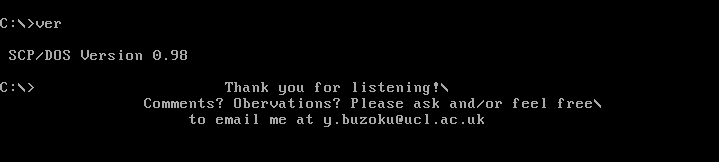
\includegraphics[width=\textwidth]{dosthanks2.png}
%	  \caption{Thank you from DOS!\,:D}
%	\end{center}
%  \end{figure}
%\end{frame}
%%%%%%%%%%%%%%%%%%%%%%%%%%%%%%%%%%%%%%%%%%%%%%%%%%%%%%%%
\begin{frame}{Muchas gracias!}
\begin{center}
Muchas gracias!

Questions? Comments? Observations? Please ask and/or feel free to email me at \url{y.buzoku@ucl.ac.uk}.
\end{center}
\end{frame}
%%%%%%%%%%%%%%%%%%%%%%%%%%%%%%%%%%%%%%%%%%%%%%%%%%%%%%%%
\begin{frame}[allowframebreaks]
	\frametitle{References}
	\nocite{*}
	\bibliographystyle{amsalpha}
	\bibliography{./refs/refs.bib}
\end{frame}
%%%%%%%%%%%%%%%%%%%%%%%%%%%%%%%%%%%%%%%%%%%%%%%%%%%%%%%%
\end{document}
